\documentclass[12pt]{article}

\usepackage{url} % websites in bib
\usepackage{hyperref}
\usepackage[a4paper,left=1in,right=1in,top=1in,bottom=1in]{geometry} % margins
\usepackage{paralist} % compact enumerates

\usepackage{graphicx}
\usepackage{caption}
\usepackage{subcaption}

\usepackage{amsmath}

\usepackage{multirow}

\usepackage{float} % figure placement

\begin{document}
	\title{}
	\author{Stefan Sebastian, 242}
	\date{}
	\maketitle
	
	\begin{abstract}
	
	\end{abstract}

	\newpage
	\tableofcontents
	\newpage
	
	\section{Introduction}
	\subsection{Motivation}
	The problem and why do I solve it
	\subsection{Related work}
	
	\section{Dataset}
	The dataset used for this experiment is a collection of beer reviews taken from the BeerAdvocate website. The original dataset was made up out of 1.5 million user reviews, from 33387 different users, collected between 1998 and 2011. It is not available at this time but I found a subset of around 500 thousand reviews on data.world\cite{BeerAdvocateData}. 
	
	The data is in csv format, each row containing various information like: beer name, beer style, alcohol content, scores for taste, appearance, aroma and a textual review. The only columns considered for this experiment were the beer style and the text review.
	
	On exploratory data analysis, 407 duplicate and 119 missing reviews were found. Also there are 104 distinct beer styles and the amount of data for each of them is quite imbalanced as can be see in figure \ref{fig:initialDistribution}, where each bar represents a beer style with a size proportional to the number of reviews for it.
	
	\begin{figure}
		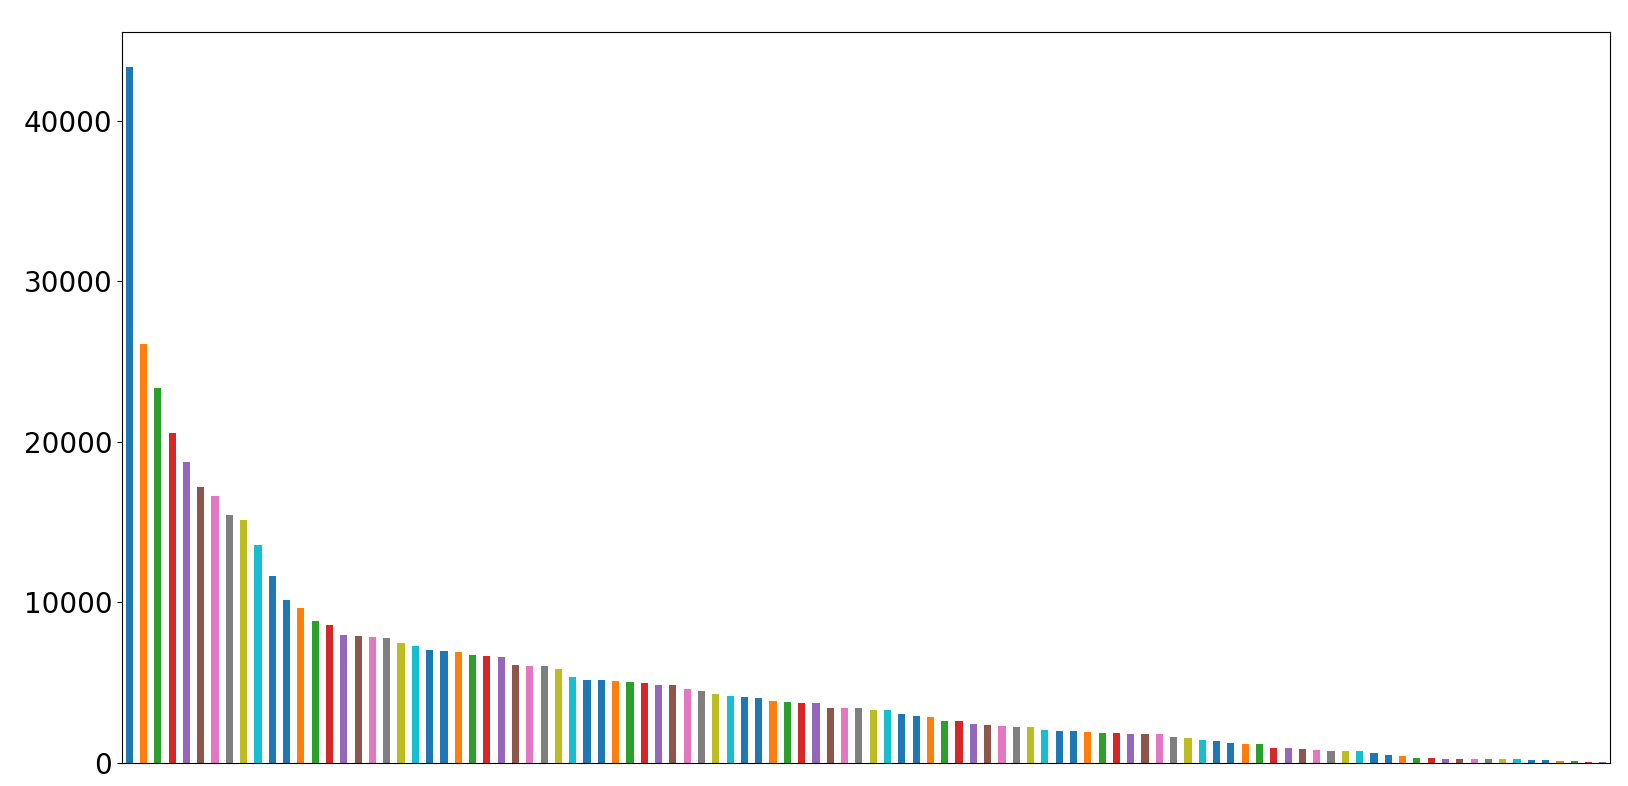
\includegraphics[width=\linewidth]{resources/InitialDistribution.png}
		\caption{A plot of the number of reviews per beer style}
		\label{fig:initialDistribution}
	\end{figure}

	The first step in preprocessing this dataset was to remove rows containing duplicates and missing values in the columns that are relevant for the experiment: beer style, text review. Next, some of the styles for which there wasn't a lot of data available were dropped, as they would be outliers for clustering. The threshold for this cut was chosen arbitrarily at 7000 reviews. 
	
	Upon inspection of the beer styles present in the dataset, a fine granularity was observed. For example, the difference between American Pale Ale and American India Pale Ale is minimal and not very rigorous. This and other similar cases would only confuse the classifier. For this reason, a mapping was made for each style to a broader category, using the taxonomy published by BusinessInsider\cite{BeerTaxonomy}. 
	
	The final mapping can be seen in figure \ref{fig:styleMapping}. Finally, a balanced dataset is built by selecting the minimum value for which we have an equal distribution of reviews per beer style, which is around 9500 per style. The analyzed dataset is made through random sampling of 9500 values for each of the remaining beer styles.
	
	\begin{figure}
		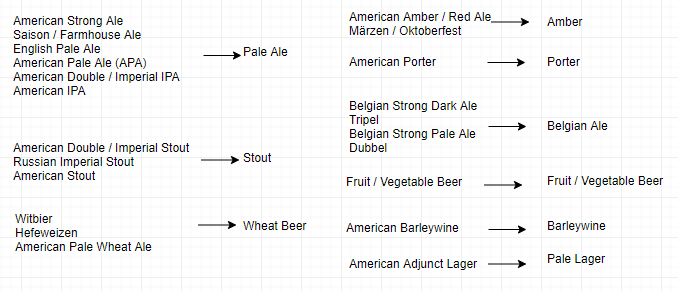
\includegraphics[width=\linewidth]{resources/MappingDiagram.png}
		\caption{Mapping of beer styles from the original dataset}
		\label{fig:styleMapping}
	\end{figure}

	\section{Solution description}
	\subsection{Model overview}
	In order to process the textual data, some features need to be extracted by using natural language processing techniques. The method used to extract numerical features about the words in the dataset is the Tf-Idf vectorizer. Tf-Idf\cite{TfIdfBook} stands for term frequency-inverse document frequency and is the most popular method for weighting term. In brief, the importance of a word is proportional to the number of times it appears in a document and inversely proportional to the number of documents it appears in. Before applying Tf-Idf, the review texts are tokenized, the stop words are removed and then each word is stemmed. Stemming is the process of reducing a word to its root, or base form, and the algorithm selected for this is the Snowball Stemmer\cite{SnowballStemmer}, which works by defining a set of rules for replacing word endings. The number of terms considered as features has been determined experimentally. Finally, the dataset contains a list of array that denotes how important is each considered term for every review.
	
	To solve the clustering problem the classic K-Means algorithm is used with two different seed initialization methods: random values and k-d trees. The first method is very simple conceptually, just choose k random points from the dataset. The second method has been described by Redmon and Heneghan\cite{KdTreeKmeans}. The basic idea is to use this data structure to divide multidimensional features into buckets and the make density estimation depending on the size of the bucket and the volume of the bounding box.
	
	The resulting clusters are evaluated based on initial beer style labels and the dominant terms in each cluster.
	
	\begin{figure}[H]
		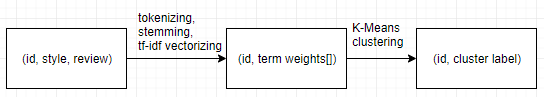
\includegraphics[width=\linewidth]{resources/model.png}
		\caption{Diagram of the transformations on the dataset}
		\label{fig:modelOverview}
	\end{figure}

	\subsection{Technologies used}
	The project was implemented in the Python programming language on the Anaconda distribution. The clustering and seed initialization algorithms were implemented from scratch.
	
	For data analysis and preprocessing the pandas\cite{Pandas} library was used, which provides some efficient data manipulation and analysis tools. The group by function was particularly useful for operations on all data of a particular beer style. 
	
	The algorithms for tokenizing and stemming were taken from the nltk library\cite{NLTK}, which is one of the most popular tools for natural language processing. The Tf-Idf vectorizer implementation was provided by the scikit-learn library\cite{sk-learn}, which contains a comprehensive collection of data analysis algorithms.
	
	In order to visualize the data and the results the following plotting tools were used. Matplotlib\cite{Matplotlib} provided a tool to make bar charts in order to observe the initial data distribution and Seaborn\cite{Seaborn} was used to generate a heatmap of the resulting clusters.
		
	\subsection{Parameters}
	The most important parameter used in the experiment is k, the number of clusters. This was chosen to be the number of distinct beer styles in the dataset, 9, as the reviews for beers of the same type should be similar to each other.
	
	The number of features for each data point is equivalent to how many word frequencies are considered. This was determined experimentally by running the basic algorithm with some different feature values. The results, shown in table \ref{tab:features}, indicate that until around 1000 there is the biggest growth in performance.
	
	\begin{center}
		\label{tab:features}
		\begin{tabular}{ |c|c|c|c| } 
			\hline
			Nr features & Precision & Recall & F1 \\
			\hline
			200 & 0.420 & 0.481 & 0.449 \\
			700 & 0.501 & 0.554 & 0.526 \\
			1000 & 0.537 & 0.532 & 0.534 \\
			1500 & 0.515 & 0.528 & 0.521 \\
			\hline
		\end{tabular}
	\end{center}

	Two methods were tested for seed initialization: random points and kd-tree based. The run with kd-trees obtained a 0.47 F1 score while, random initialization got a 0.53 F1 score. This might be caused by finding good starting points through randomness or that the large number of features is not a good fit for the kd-tree data structure.

	\section{Evaluation}
	\subsection{Metrics}
	The direction chosen for evaluation is how well the clusters found separate the initial dataset by beer types. In order to do this, each cluster is labeled with the most common style of beer among its elements. This turns our problem intro a multi-label classification one.
	
	The metrics used are the ones described by Beleites at al.\cite{MultilabelClassification} for multi-class problems. First of all, a confusion matrix is computed, which is a \(lxl\) matrix where l is the number of features. Each element (x, y) in the confusion matrix has a value meaning how many times a data point with label x has been classified as having label y. Precision and recall are then calculated for each label, simulating the binary evaluation. 
	
	Precision, also called positive predictive value, is a fraction that represents how many elements classified with a label have been assigned correctly. Recall, also known as sensitivity, is the fraction of instances correctly assigned to a class and all instances from that class. For the binary case, precision and recall can be calculated as in figure \ref{eq:PrecRecall}, where tp, fp, fn stand for true positives, false positives and false negatives. This can be extended to the confusion matrix, for each row, as follows: precision is the fraction of the value on the diagonal and the sum of values on the column, recall is the value on the diagonal divided by the sum of values on the row. The precision and recall of the multi-label classifier can then be computed as the means of the values obtained from the previous step.
	
	\begin{equation}
	\label{eq:PrecRecall}
	precision = \frac{tp}{tp + fp} \quad recall = \frac{tp}{tp + fn}
	\end{equation}
	
	F1 score is a combined measure of precision and recall, used to provide a single measurement for the system. It represents the harmonic mean of the two values, as in figure \ref{eq:F1}, where mp and mr are mean precision and mean recall.
	
	\begin{equation}
	\label{eq:F1}
	F1 = \frac{2 * mp * mr}{mp + mr}
	\end{equation}
	
	\subsection{Results}
	\subsubsection{Multi-label classification score}
	The correlation between the beer styles of the data points and the type that is most prevalent in the resulting clusters was chose as a measure of evaluation. For the best run, the result can be seen in table \ref{tab:results}. These were obtained using the random seed initialization method.
	
	\begin{center}
		\label{tab:results}
		\begin{tabular}{ |c|c| } 
			\hline
			Mean precision & 0.537 \\
			Mean recall & 0.532 \\
			F1 score & 0.534 \\
			\hline
		\end{tabular}
	\end{center}

	\subsubsection{Heatmap}
	In order to better visualize the results a heatmap was generated. Visible in figure \ref{fig:heatmap}, the diagram helps visualize which style of beer is more common in which cluster. As expected, there is a clear separation for most of the dominant styles in each cluster. This is best observed for the following cluster, style pairs: 0 with Porter, 1 with Stout, 2 with Pale Lager, 4 with Wheat Beer, 5 with Belgian Ale, 6 with Fruit/Vegetable Beer and 7 with Barleywine. For cluster 3 there are two dominant classes : Pale Ale and Amber, which can be explained by the fact that Amber is a particular style of ale. For cluster 8 there is no clear majority, meaning it might be a collection of outliers from other styles.
	
	\begin{figure}
		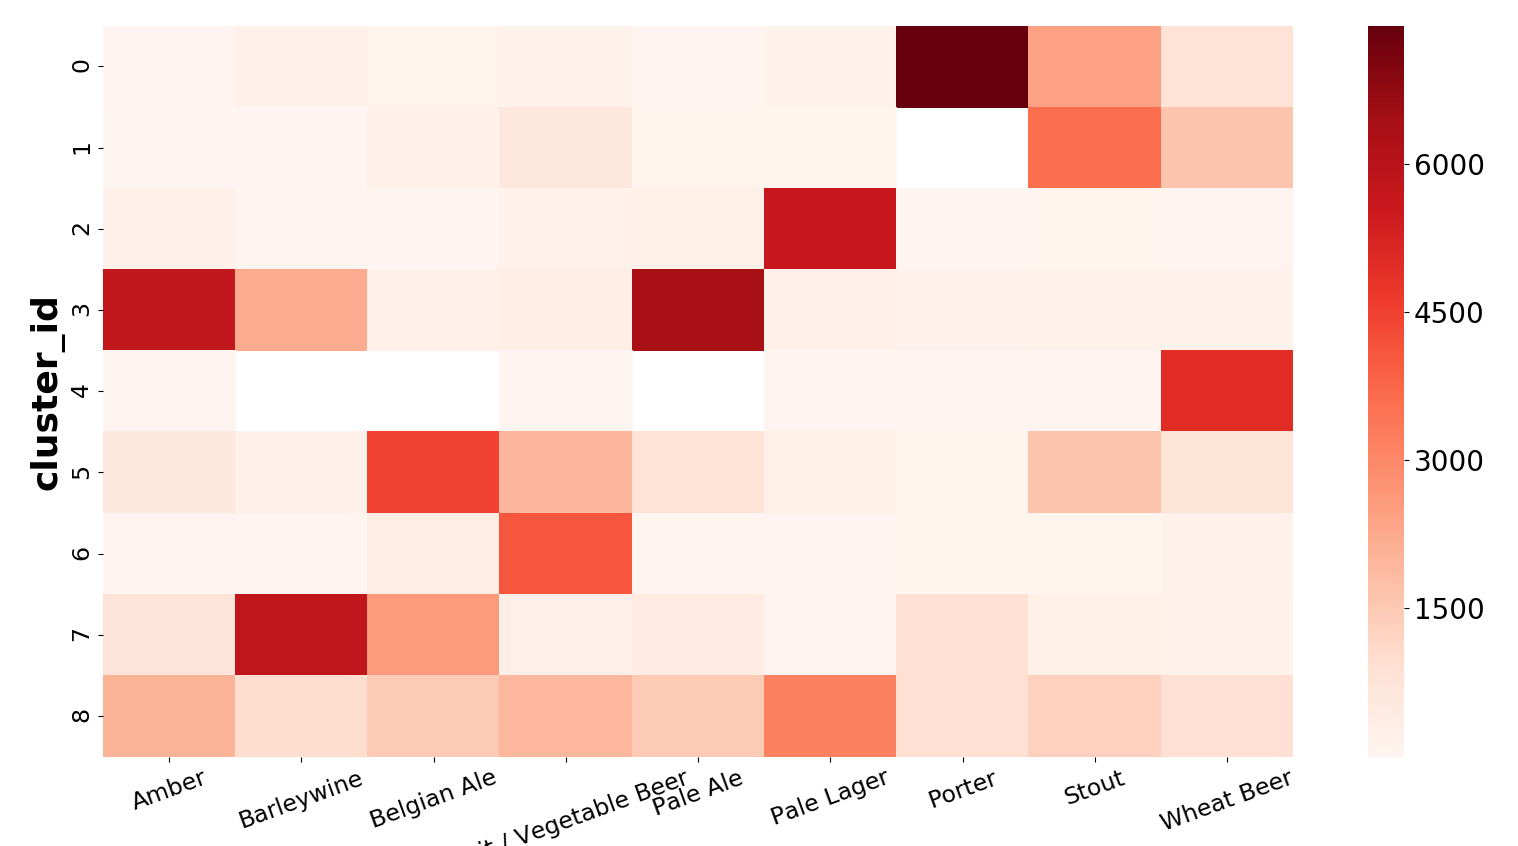
\includegraphics[width=\linewidth]{resources/9500rheatmap.png}
		\caption{Heatmap of beer styles per cluster}
		\label{fig:heatmap}
	\end{figure}
	
	\subsubsection{Common words per cluster}
	In order to interpret what features these clusters have in common, we can look at the most popular words for each cluster, identified by id. Figure \ref{fig:words} shows the 10 words with the highest tf-idf score for the mean of each cluster. Looking at this figure we can find the reason for the shape of cluster 8, as the most common words are general words used in beer description, like 'beer', 'taste', 'drink', 'flavour', which can be applied to any beer style. 
	
	Another thing we can observe from the table of common words is the difference between 'Porter' and 'Stout' styles, which are often put under the same category. According to the diagram, Porter beers tend to have a stronger chocolate, roast, coffee taste while Stouts also have a fruity, citrus taste.
	
	An interesting observation is that while the Wheat Beer style is clearly associated with cluster number 4, the feature words for this cluster: 'chocolate', 'dark', 'roast' are not at all representative of the style.
	
	\begin{figure}
		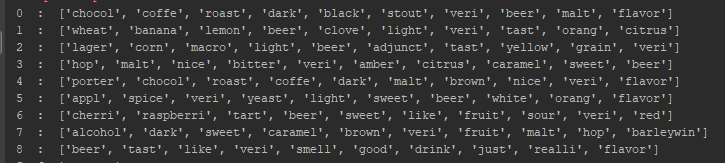
\includegraphics[width=\linewidth]{resources/words.png}
		\caption{Most common words for each cluster}
		\label{fig:words}
	\end{figure}
	
	\section{Conclusions}
	
	\newpage
	\bibliography{references_document}
	\bibliographystyle{ieeetr}
\end{document}